\section{Introduction}
\label{sec:intro}

\FIXME{Here is a reference to make sure that citations are working~\cite{Bugbee16,bblmw19}.}

Energy consumption due to buildings (both residential and commercial)
is estimated to be 20\% to 40\% of the total energy usage in
developed countries~\cite{pop08}, and
lighting and heating are two significant components of this demand~\cite{keh05}.
Natural light (i.e., sunlight) is a readily available resource that
can contribute both to the illumination~\cite{Leslie03}
and to the heating~\cite{Lunde80} of structures.
Further, the use of natural light for plant growth is dramatically more
energy efficient than artificial lighting~\cite{Bugbee16}. \FIXME{Need reference.}

We propose to investigate how to utilize actively
controlled catoptric (mirror) surfaces effectively for improved illumination,
plant growth, and heating of buildings.  Through computer-based control of
the dynamic positioning of
individual mirrors, and cyber-physical integration of the mirrors,
the devices
that orient them, and customized objectives and
constraints,
we propose to enable fine-grained management of sunlight as a resource.

Figure~\ref{fig:amp} shows a prototype catoptric surface (called AMP) that was 
designed, fabricated, and installed during an undergraduate architecture studio 
taught by Co-PI C.~Ahrens. The installation redirects light from gable ends of an 
existing building into the darker recesses of the atrium.

\begin{figure}[ht]
\centering
\subfloat[\mbox{ }]{
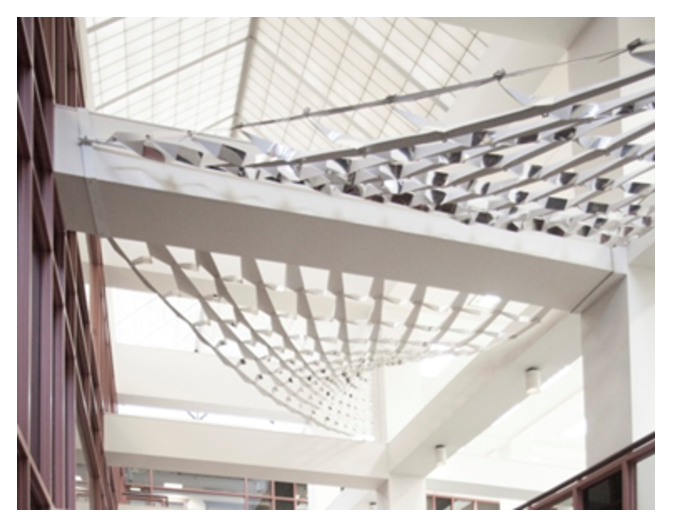
\includegraphics[width=0.45\linewidth]{figures/amp}
\label{fig:amp}}
\qquad \qquad
\subfloat[\mbox{ }]{
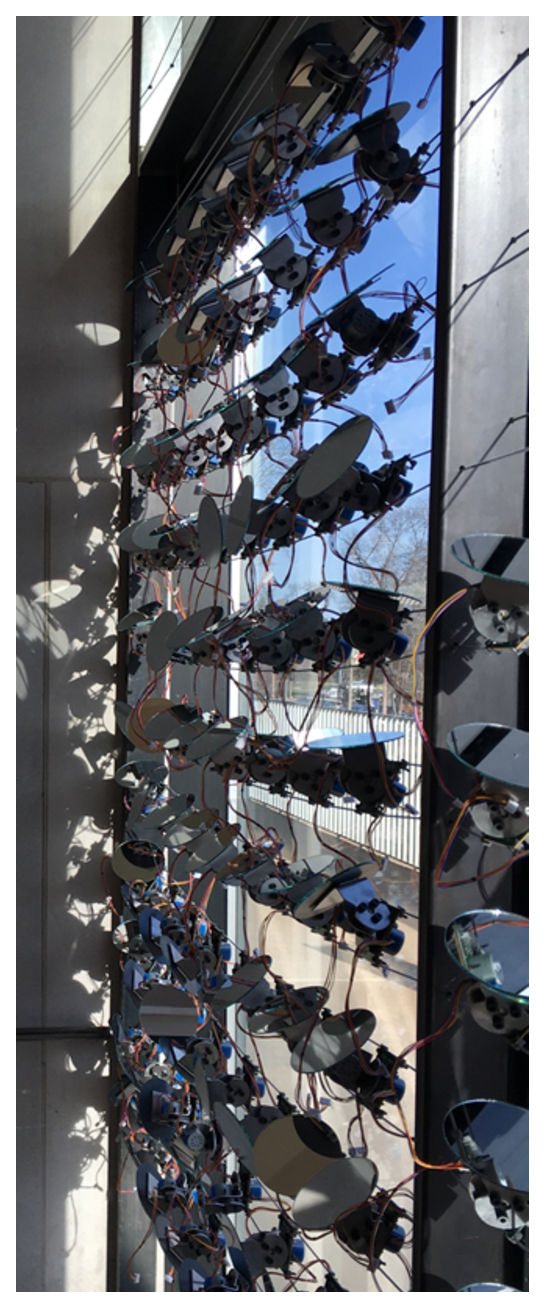
\includegraphics[width=0.14\linewidth]{figures/steinberg}
\label{fig:steinberg}}
\caption{Catoptric system prototypes.
(a)~\emph{AMP}, TRex building, St.~Louis.
(b)~Steinberg Hall, St.~Louis.
}
\label{fig:proto}
\end{figure}

We are now developing a
new version in which over 600 mirrors are under 
active, 2-axis control and therefore the mirrors
can be pointed in different directions dynamically as desired over time. 
This next-generation installation is currently under construction within 
the south wall of the Steinberg Hall atrium on the campus of 
Washington University in St.~Louis; a subset of the mirrors in this new
installation is shown in Figure~\ref{fig:steinberg}.

The community with which we will collaborate on this effort is
the 39~North AgTech Innovation District in St.~Louis County. Under the
supervision of the county and the St.~Louis Economic Development Partnership, 
a master plan has been prepared to develop the area in the vicinity of  
anchor institutions Bayer AG and the Donald Danforth Plant Science Center. 
